\documentclass[letterpaper,twoside,12pt]{article}

\usepackage[USenglish]{babel} 
\usepackage[T1]{fontenc}
\usepackage{lmodern} 
\usepackage[top=1.5in, bottom=1.5in, left=1in, right=1in]{geometry}
\usepackage{amsmath}
\usepackage{graphicx}
\usepackage{enumerate}
\usepackage{setspace}
\usepackage{arydshln}
\usepackage{caption}
\usepackage{subcaption}
\usepackage[bitstream-charter]{mathdesign}
\usepackage{setspace}
\usepackage[round]{natbib}
\usepackage{soul}
\setlength{\belowcaptionskip}{12pt}
\usepackage{framed}
\usepackage{rotating}
\usepackage{hyperref}
\usepackage[hang,flushmargin]{footmisc} 
\usepackage{framed}
\usepackage{arydshln}
\usepackage{endnotes}
\usepackage{arydshln}
\usepackage{comment}
\usepackage{url}
\usepackage{pdflscape}
\usepackage{longtable}
\usepackage[capposition=top]{floatrow}
\usepackage{subcaption}
 \raggedbottom
\providecommand{\keywords}[1]{\textbf{Keywords:} #1}

\usepackage[latin1]{inputenc}
\doublespace

\newcommand*{\SuperScriptSameStyle}[1]{%
  \ensuremath{%
    \mathchoice
      {{}^{\displaystyle #1}}%
      {{}^{\textstyle #1}}%
      {{}^{\scriptstyle #1}}%
      {{}^{\scriptscriptstyle #1}}%
  }%
}

\newcommand*{\oneS}{\SuperScriptSameStyle{*}}
\newcommand*{\twoS}{\SuperScriptSameStyle{**}}
\newcommand*{\threeS}{\SuperScriptSameStyle{*{*}*}}

\newcommand{\eeq}{\end{equation}}
\newcommand{\vs}{\vspace{5mm}}
\newcommand{\vsmore}{\vspace{15mm}}
\newcommand{\letters}{\begin{enumerate}[a.]}
\renewcommand{\i}{\item}
\renewcommand{\u}{\underline}
\renewcommand{\footnotelayout}{\doublespacing}
\renewcommand{\baselinestretch}{2}
\renewcommand{\footnotesize}{\normalsize
\setlength{\footnotesep}{\baselineskip}} 
\newenvironment{nscenter}
 {\parskip=0pt\par\nopagebreak\centering}
 {\par\noindent\ignorespacesafterend}
% \let\footnote=\endnote

%--------------------------------------------------------
\begin{document}
\title{Online Appendix: Graphical Presentation of Regression Discontinuity Results}
\date{}

\maketitle

\clearpage
\listoffigures

\setcounter{figure}{0} \renewcommand{\thefigure}{A.\arabic{figure}}


\clearpage
\begin{figure}
  \caption{Mean vote share difference between winners and losers by Democratic margin of victory in previous election, from 1942 to 2008.}\label{fig:main_polynomial}
\vspace{-1mm}
  \centerline{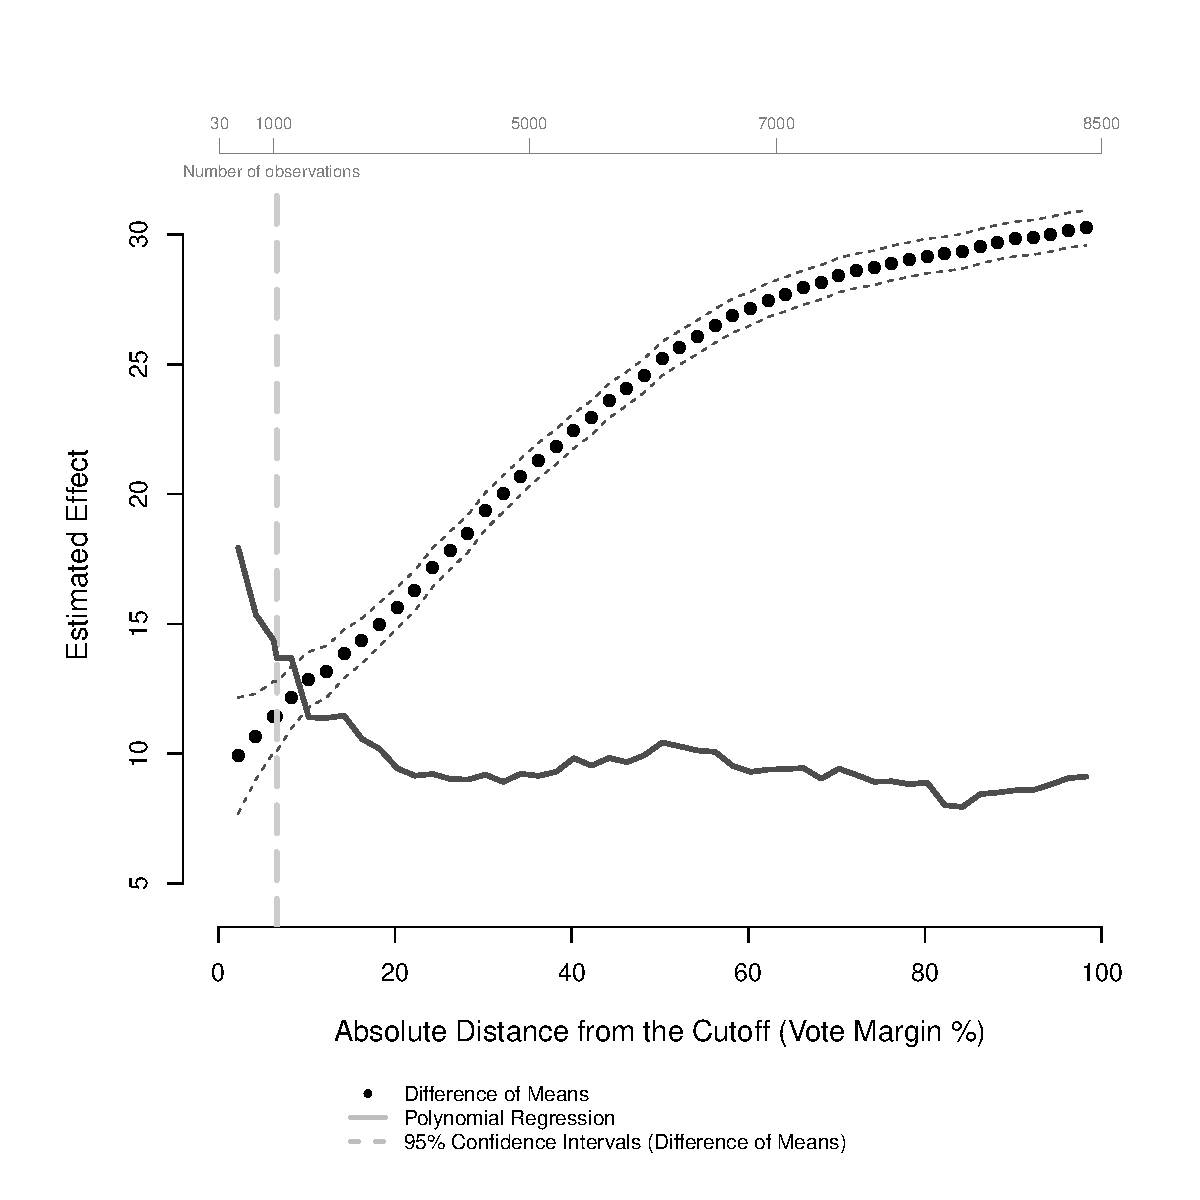
\includegraphics[width=1\textwidth]{with_add_est_plot_poly.pdf}}
  \floatfoot{Note: Dashed gray line at the optimal bandwidth estimated by the method of \citet{imbens2011optimal}. Differently than our plots in the main text, we present results for the the entire range of the running variable because it is common practice in regression-discontinuity designs that use polynomial regression models to use the full dataset.}
  \end{figure}
\clearpage

\begin{figure}
  \caption{Mean standardized vote share difference between winners and losers by Democratic margin of victory in previous election, from 1942 to 2008}\label{fig:main_est}
\vspace{-1mm}
  \centerline{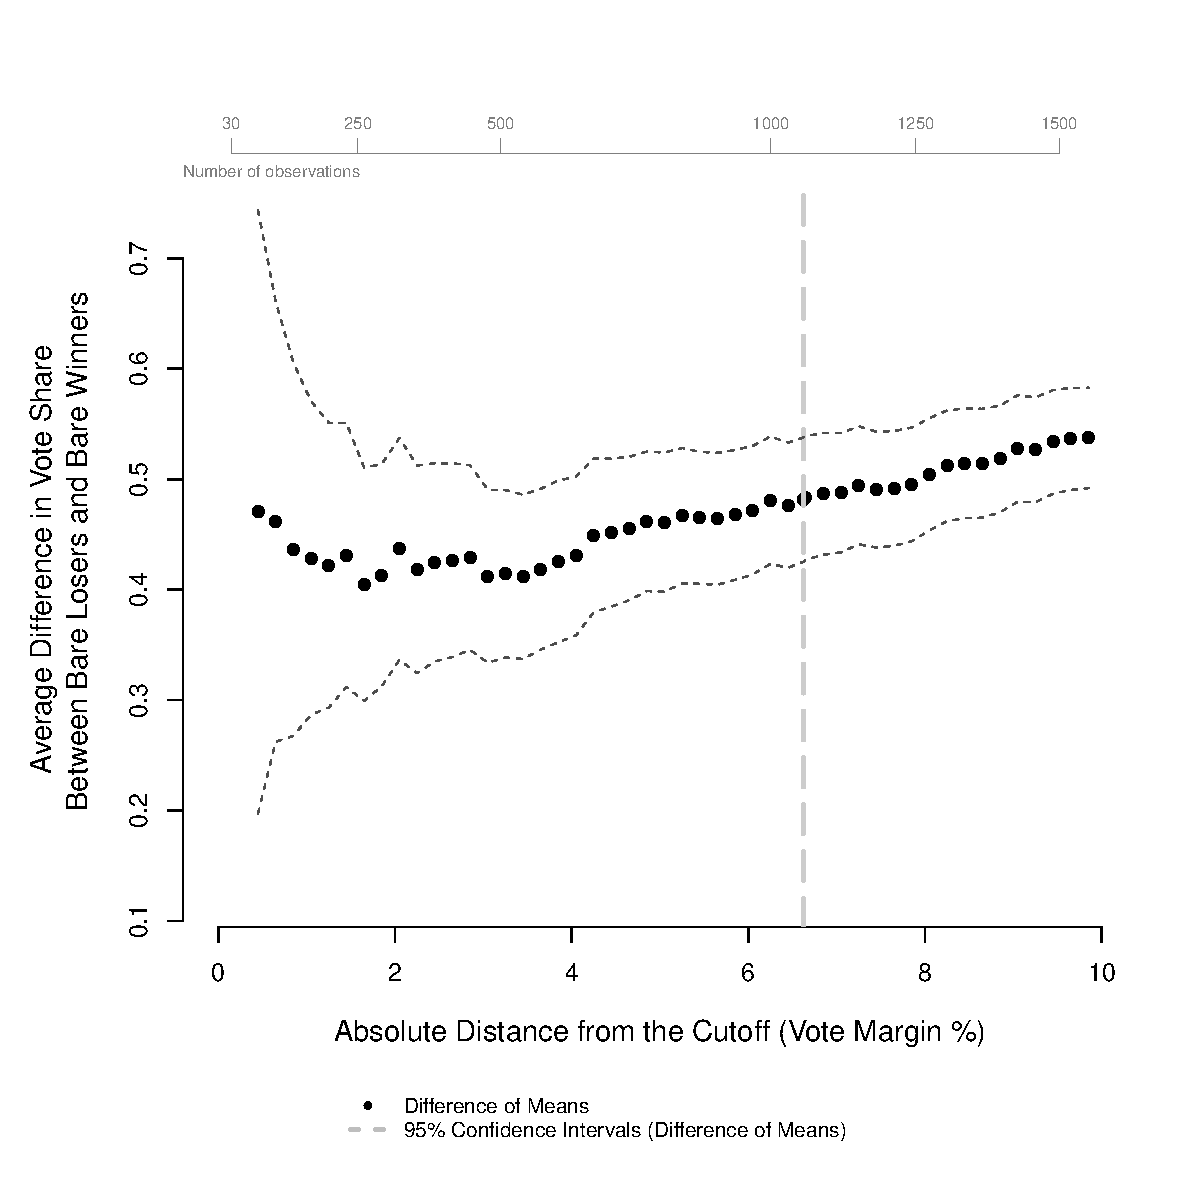
\includegraphics[width=1\textwidth]{no_add_est_plot_standardized.pdf}}
  \floatfoot{Note: Dashed gray line at the optimal bandwidth estimated by the method of \citet{imbens2011optimal}.}
  \end{figure}
\clearpage


\clearpage
\begin{figure}
\caption{Tests for balance: Standardized difference of means of pre-treatment covariates by Democratic margin of victory (95\% confidence intervals).}\label{fig:balancepartial_12}
 \vspace{-1mm}
   \centerline{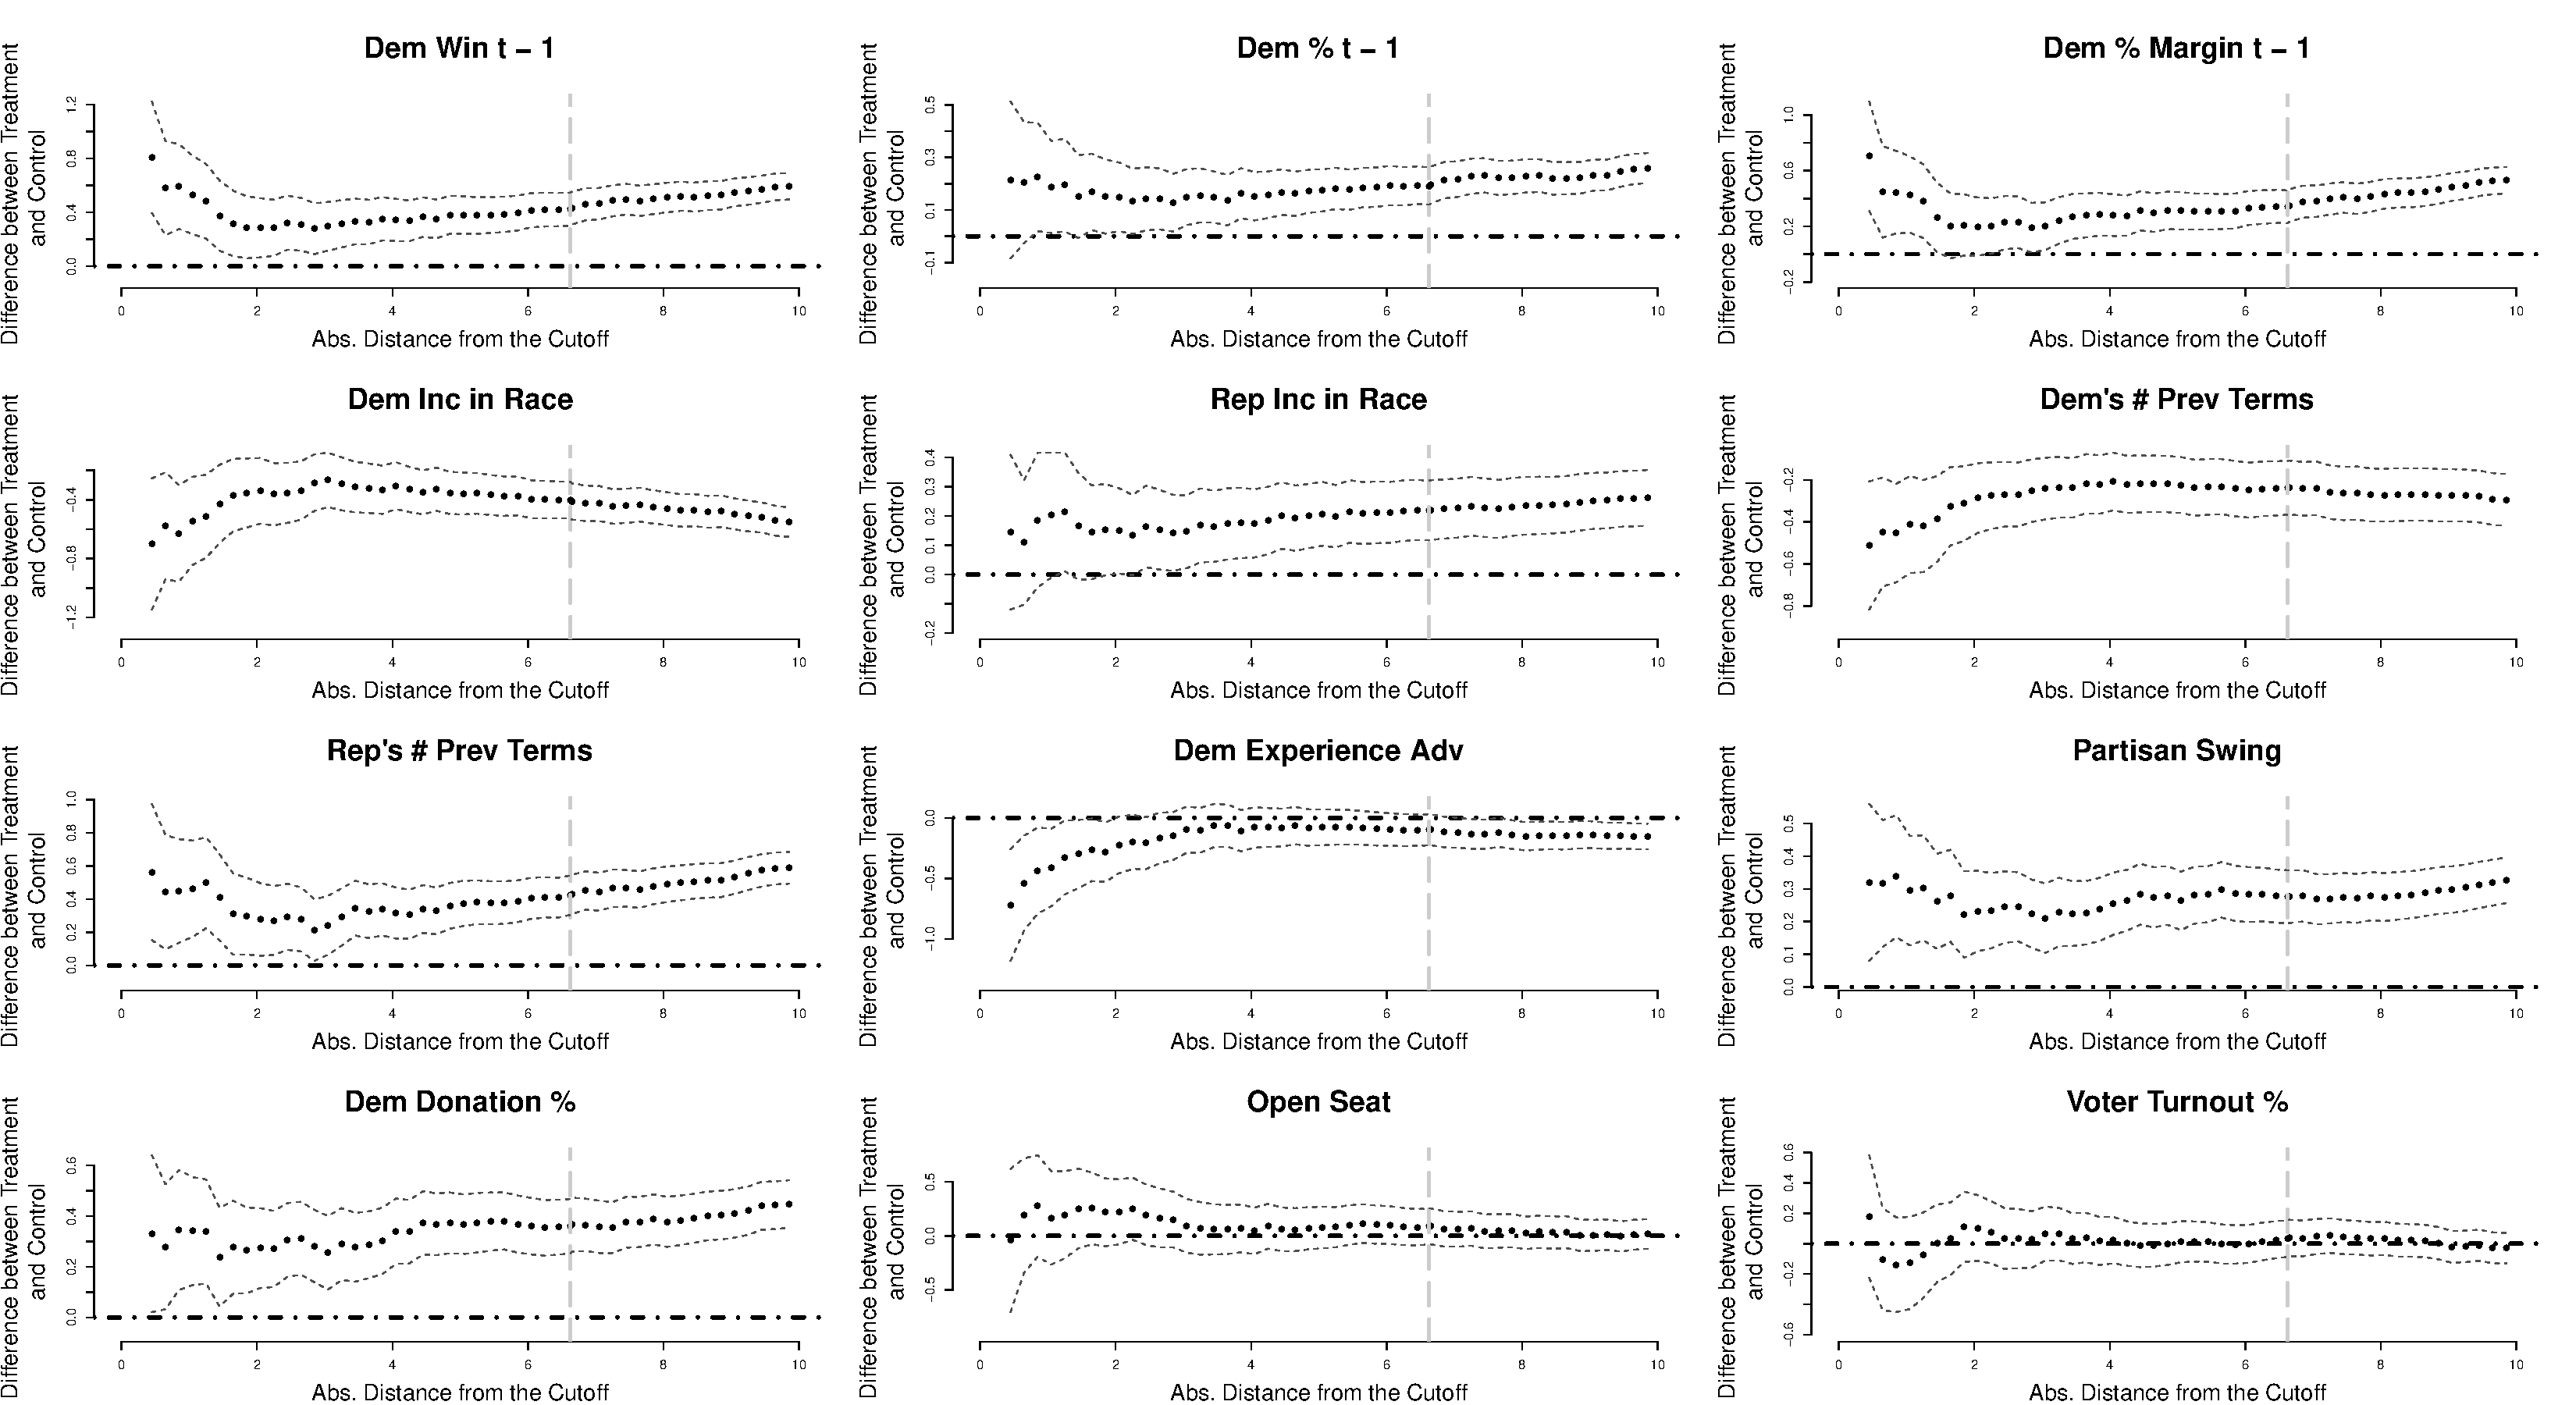
\includegraphics[width=1\textwidth]{balance_plots_12.pdf}}
   \floatfoot{Note: Dashed gray line at the optimal bandwidth estimated by the method of \citet{imbens2011optimal}. U.S.\ House of Representatives, from 1942 to 2008.}
    \end{figure}
\clearpage


\clearpage
\bibliographystyle{apsr}	
\bibliography{RDnote}


\end{document}
